\documentclass[letterpaper,openany,twoside,twocolumn]{book}
%\documentclass[a4paper,openany,oneside,twocolumn]{book}

\newcommand{\PATH}{../../}

\usepackage[justified]{\PATH dndtemplate/dnd}

\usepackage{\PATH classes/stylesheet/classes_stylesheet}
\usepackage{\PATH classes/stylesheet/classes_commands}
\usepackage{\PATH classes/stylesheet/classes_variables}
\usepackage{\PATH classes/stylesheet/shadowfy}
\usepackage{\PATH classes/stylesheet/ornamented}

\usepackage[english]{babel}
\usepackage[utf8]{inputenc}

%\newcommand{\entryfont}{\DndFontStatBlockBody} & uses the default font provided by the LaTeX DnD-Template
\newfontfamily\entryfont{Kalam}[Path=\PATH template/fonts/,Extension=.ttf,UprightFont=Kalam-Regular,BoldFont=Kalam-Bold] % requires XeLaTeX or LuaTeX
\newfontfamily\titlefont{Modesto Bold}[Path=\PATH template/fonts/,Extension=.ttf,UprightFont=Modesto Bold,BoldFont=Modesto Bold] % requires XeLaTeX or LuaTeX

\ClassName{Advisor}

\begin{document}
	% Titlepage	
	\classesTitlePage{The Advisor}{images/titlepage_Advisor.jpg}{0cm}{-2cm}{min width=\paperwidth, min height=\paperheight}{https://www.artstation.com/artwork/arZ4R}{Piri Reis}{Guan Ye Chen}
	
	\begin{tikzpicture}[remember picture, overlay]
		\node[opacity=1,inner sep=0pt, anchor=north east, xshift=4cm] at (current page.north east){
\includegraphics[height=0.5\paperheight, keepaspectratio]{images/Advisor(1).png}};
		\addImageDBEntry{Page 2}{Background Art}{https://cdn.artstation.com/p/assets/images/images/000/697/528/large/tj-foo-grand-library.jpg?1431011034}{Grand Library}{TJ Foo}
		\node[opacity=1,inner sep=0pt, xshift=6cm, yshift=-1cm] at (current page.center){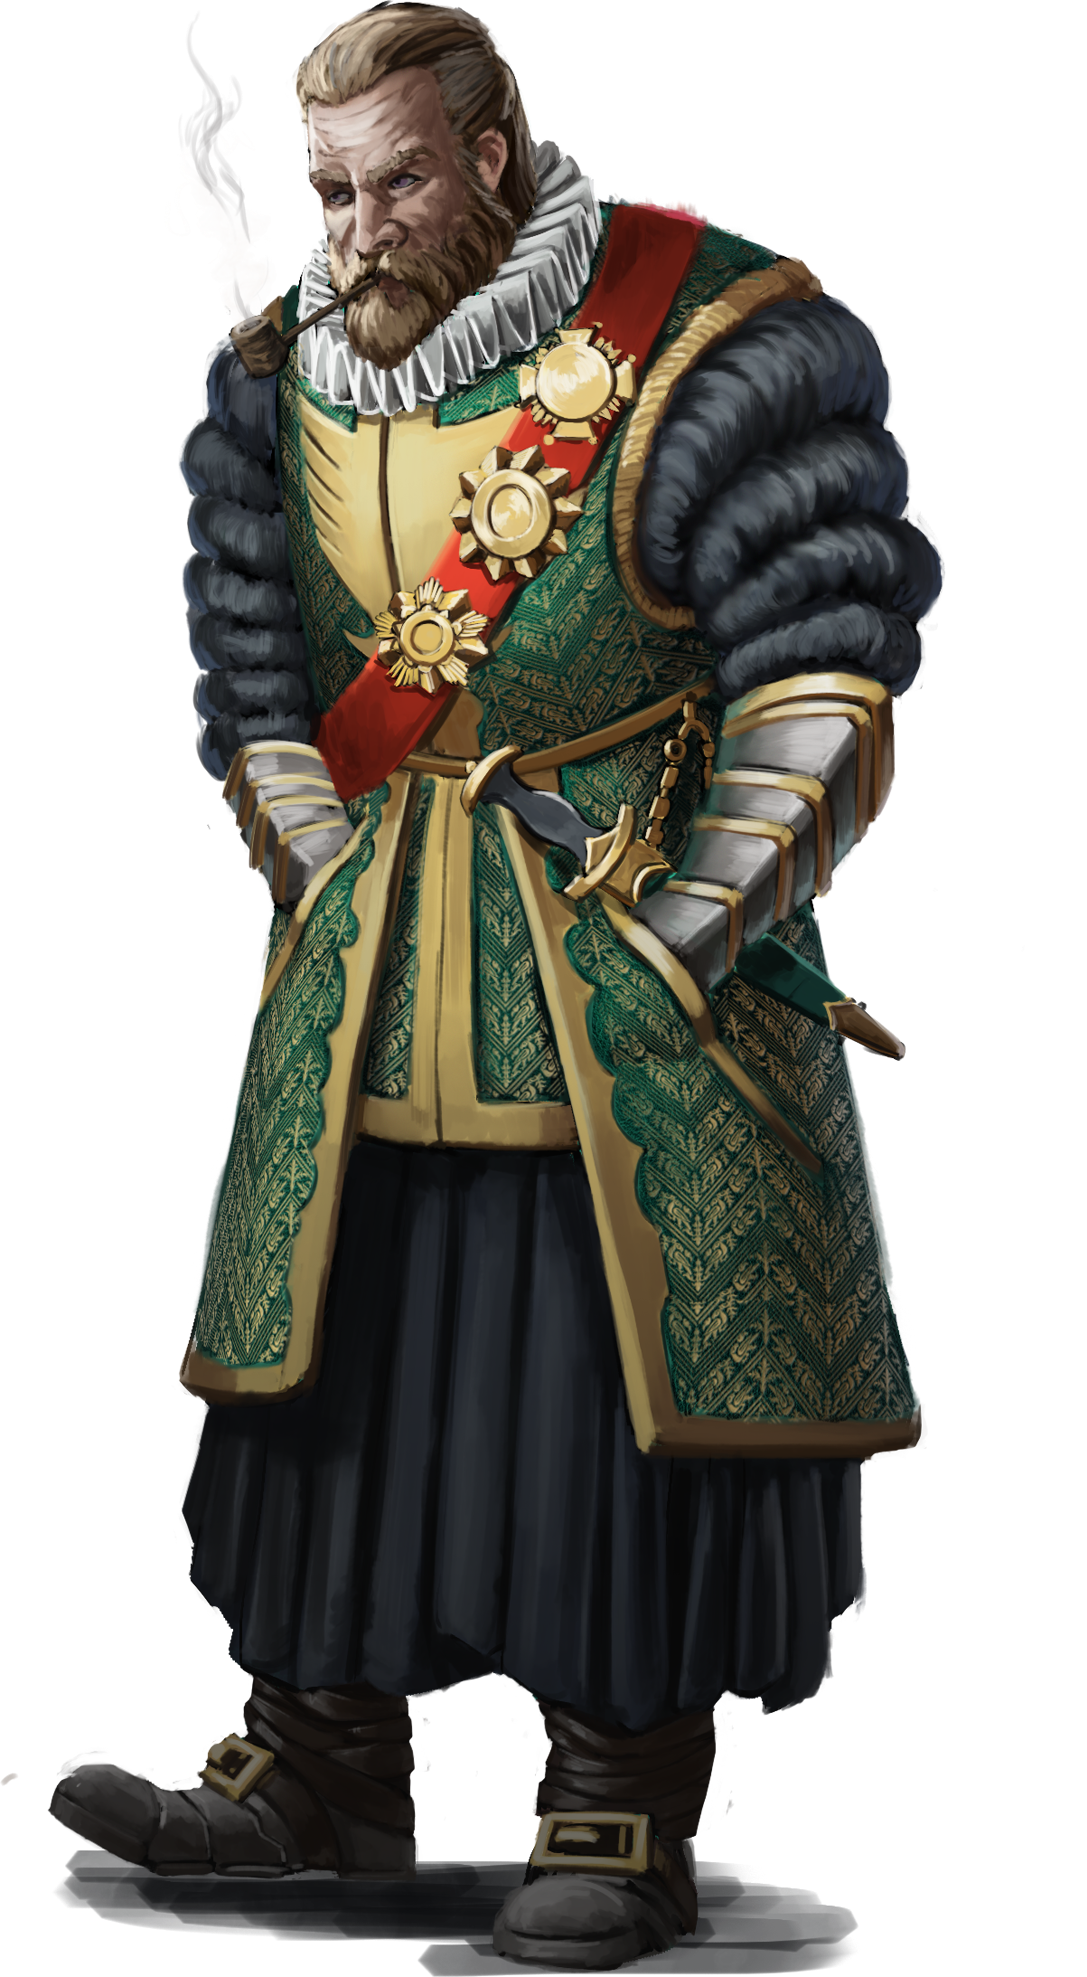
\includegraphics[height=0.5\paperheight, keepaspectratio]{images/Advisor(2).png}};
		\addImageDBEntry{Page 2}{Character Art}{https://www.behance.net/gallery/54878727/Empires-in-ruins-Main-Characters}{Empires in Ruins - Main Characters}{Konrad Langa}
	\end{tikzpicture}
	\vspace*{-2.4\fontdimen6\font}
	\section*{Advisor}
	\entryfont The young elven woman's eyes\\light up with joy as soon as she\\steps through the tall and meticulously\\-crafted door into the magnificent study.\\Reverently, she runs her fingers across each\\page of ancient tomes, a treasure trove of old\\magics and invaluable guidance for the future.

	In a war room adorned with weapons and\\armor, a dwarven general directs the\\movement of war pieces with a croupier\\stick. Clad in sturdy plate armor, the commander\\demands silence from the room. Amidst the\\tension, the general carefully weighs the options before uttering two decisive words: \textbf{"TO WAR!"}

	Amidst the shifting stones of an archaic structure, a tomb opens its secrets to a grizzled half-orc. Years of study and exploration culminate in this moment of triumph as he deciphers the hidden pattern and unlocks its authenticity.

	These are the defining moments for members of the Advisor class — individuals brimming with knowledge and wisdom, adept at offering guidance and support. An Advisor represents the pinnacle of expertise and versatility, proficient in teaching allies and others alike.
	\subsection{Masters of the Mundane}
	In an archetype often dominated by magical prowess, the Advisor stands out as a master of their chosen expertise. Whether honed through rigorous schooling or innate academic brilliance, they ascend to the highest echelons alongside their arcane counterparts.

	While not traditionally known for their physical strength or dexterity, the Advisor exudes remarkable versatility. They possess the uncanny ability to unravel ancient riddles and calculate the precise down-swing required for a weapon strike. In a perpetual cycle of learning and teaching, Advisors continually expand their knowledge and share their wisdom with others.
	\subsection{Edge of Education}
	In many respects akin to Bards, not every teacher or professor can claim the title of a true Advisor. It is a formidable challenge for most to distill complex truths and vast knowledge into concise, meaningful advice. To comprehend the weight, intricacies, and nuances of diverse subjects and then convey them in a clear and understandable manner is an accomplishment akin to performing magic.

	Drawing upon their extensive knowledge and the wisdom of countless others, Advisors become masters of their chosen pursuits. The relentless pursuit of knowledge, mastery of a craft, or the perfection of an art propels them forward, driven more by their thirst for understanding than any rigid ideology.
	\vfill\eject
	\vspace*{20cm}
	\subsection{Creating an Advisor}
	As you make your Advisor character, the largest focus should be put onto what you want the character's Field of Expertise to be. Although the class features related to your Field of Expertise don't appear until you reach 3rd level, plan ahead by reading their descriptions at the end of the class.
	\clearpage
	\noindent Not all Advisors got to be one due to an equal playing field, though. It's essential to consider your character's upbringing and background. Were they enrolled in the most prestigious, high-brow, and curricularly extensive institution this side of the Forgotten Realms? Were they part of a prestigious lineage, with access to ancient knowledge and arcane secrets? Alternatively, did they learn to live on their own, increasing their survival skills, with each passing day, mastering the arts of self-reliance and adaptability? The path they took before embracing the mantle of an Advisor can significantly influence their worldview, motivations, and capabilities.
	
	\sectionQuickBuild{Intelligence}{Constitution or Dexterity}{Sage}{}
	
	\sectionMultiClass{Intelligence}{13}{}{light armor, one skill of your choice, and one set of artisan's tools of your choice}
	
	\section*{Class Features}
	As an Advisor, you gain the following class features
	
	\sectionHitPoints{6}
	
	\subsubsection*{Proficiencies}
	\textbf{Armor:} Light armor, medium armor\\
	\textbf{Weapons:} Simple weapons, hand crossbows, shortswords\\
	\textbf{Tools:} Choose any two\\\\
	\textbf{Saving Throws:} Intelligence, Wisdom\\
	\textbf{Skills:} Choose any four
	
	\subsubsection*{Equipment}
	You start with the following equipment, in addition to the equipment granted by your background:
	\begin{itemize}
		\item (a) a shortbow and quiver of 20 arrows or (b) any simple weapon
		\item (a) a book or (b) a case for maps or scrolls
		\item (a) a diplomat’s pack or (b) an entertainer's pack
		\item Leather armor, a handaxe and a scholar's pack
	\end{itemize}
	
	\begin{adjustwidth}{-1em}{-1.5em}\begin{ornamentedbox}
	\begin{DndTable}[width=\linewidth, header=The Advisor]{llXr}
		\textbf{Level}  	&\makecell[l]{\textbf{Proficiency} \\ \textbf{Bonus}}	&\textbf{Features}					&\makecell[r]{\textbf{Advice} \\ \textbf{Die}}\\
		1st					&\multicolumn{1}{c}{+2}		&Expertise, Word of Advice			&1d4				\\
		2nd					&\multicolumn{1}{c}{+2}		&Common Knowledge, Master of One	&2d4				\\
		3rd					&\multicolumn{1}{c}{+2}		&Field of Expertise					&3d4				\\
		4th					&\multicolumn{1}{c}{+2}		&Ability Score Improvement			&4d4				\\
		5th					&\multicolumn{1}{c}{+3}		&True Abettor						&5d4				\\
		6st					&\multicolumn{1}{c}{+3}		&Field of Expertise Feature			&6d4				\\
		7nd					&\multicolumn{1}{c}{+3}		&Your Own Advice					&7d4				\\
		8rd					&\multicolumn{1}{c}{+3}		&Ability Score Improvement			&8d4				\\
		9th					&\multicolumn{1}{c}{+4}		&Cut to the Chase					&9d4				\\
		10th				&\multicolumn{1}{c}{+4}		&Field of Expertise Feature			&10d4				\\
		11th				&\multicolumn{1}{c}{+4}		&Repeated Mantra					&11d4				\\
		12th				&\multicolumn{1}{c}{+4}		&Ability Score Improvement			&12d4				\\
		13th				&\multicolumn{1}{c}{+5}		&Insult to Injury					&13d4				\\
		14th				&\multicolumn{1}{c}{+5}		&Field of Expertise Feature			&14d4				\\
		15th				&\multicolumn{1}{c}{+5}		&Common Knowledge (3 Creatures)		&15d4				\\
		16th				&\multicolumn{1}{c}{+5}		&Ability Score Improvement			&16d4				\\
		17th				&\multicolumn{1}{c}{+6}		&Louder Than Words					&17d4				\\
		18th				&\multicolumn{1}{c}{+6}		&Field of Expertise Feature			&18d4				\\
		19th				&\multicolumn{1}{c}{+6}		&Ability Score Improvement			&19d4				\\
		20th				&\multicolumn{1}{c}{+6}		&Unforgettable Instruction			&20d4				\\
	\end{DndTable}
	\end{ornamentedbox}\end{adjustwidth}
	
	\subsection*{Expertise}
	At 1st level, choose two of your skill proficiencies, or one of your skill proficiencies and one of your tool proficiencies. You gain expertise (double proficiency bonus) for the chosen skills.
	
	\begin{tikzpicture}[remember picture, overlay]
		\node[opacity=1,inner sep=0pt, anchor=south east, yshift=-0.5cm, xshift=-1cm] at (current page.south east){
\includegraphics[width=0.5\paperwidth, keepaspectratio]{images/Advisor(3).png}};
		\addImageDBEntry{Page 3}{Art}{https://www.artofmtg.com/art/kambal-consul-of-allocation/}{Kambal, Consul of Allocation MtG Art from Kaladesh}{Vincent Proce}
	\end{tikzpicture}
	
	\newpage
	\subsection*{Word of Advice}
	At 1st level, you can utilize your vast knowledge to aid others. Whenever a creature, other than yourself, that can hear you, makes an ability check or saving throw with an ability you are proficient in, you can use your reaction and expend one of your Advice Die. Roll the die and add or subtract the result to their roll. Intelligence is your ability for these effects when you use this trait.
	
	\subparagraph*{Advice Dice} At 1st level, you possess one advice die, which is a d4. You gain more as you reach higher levels, as shown in the Advice Die column of the Advisor table.
	
	You can never have more advice dice than what is specified in the Advisor table for your current level. Each time you provide guidance or support by using an advice die, it is expended. You regain all of your expended advice dice when you finish a long rest.
	
	\subparagraph*{Saving Throws} When you choose to subtract the number rolled, the target can choose to make an Intelligence saving throw to avoid following your word’s effects. The saving throw DC is calculated as follows:
	\begin{center}
		\textbf{Advice Save DC} = 8 + your Proficiency Bonus + \\your Intelligence Modifier
	\end{center}
	
	\sidebarOptionalRule{Alternate Advice}{%
		During the character building process you can choose that your Advisor gives advice based on previous experience and wisdom, or charismatic communication. The Word of Advice ability modifier can therefore be changed to use Intelligence, Wisdom, or Charisma.
	}%
	
	\subsection*{Common Knowledge}
	At 2nd level, your teachings can assist in all sorts of future tasks. Whenever you finish a short or long rest, you can choose one skill or tool proficiency that you have and grant it to a friendly creature. They lose this proficiency when you use this feature to choose a different proficiency that you have. Starting at 15th level, you can grant this to up to 3 friendly creatures.
	
	\subsection*{Master of One}
	Starting at 2nd level, choose one of your skill or tool proficiencies. Whenever you make an ability check that uses the chosen proficiency, you can treat a d20 roll equal to or lower than your Intelligence modifier to be equal to your modifier plus 1.
	
	\subsection*{Field of Expertise}
	At 3rd level, you choose a Field of Expertise that you utilize in the application of your Advisor abilities: Arcanology, Archeology, Criminology, Polemology, Theology or Zoology - detailed at the end of the class description. Your archetype choice grants you features at 3rd level and then again at 6th, 10th, 14th and 18th level.
	
	\subsection*{Ability Score Improvement}
	When you reach 4th level, and again at 8th, 12th, 16th, and 19th level, you can increase one ability score of your choice by 2, or you can increase two ability scores of your choice by 1. As normal, you can’t increase an ability score above 20 using this feature.
	
	Using the optional feats rule, you can forgo taking this feature to take a feat of your choice instead.
	
	\subsection*{True Abettor}
	Starting at 5th level, your quick thinking and drive to protect yourself allows you to assist in other ways, from a distance. You can take a bonus action on each of your turns in combat. This action can be used only to take the Disengage, Help or Search action.
	
	Additionally, when you use the Help action to aid an ally in attacking a creature, the target of that attack can be within 30 feet of you, rather than within 5 feet of you, if the target can hear you.
	
	\subsection*{Your Own Advice}
	Beginning at 7th level, follow through on your words. You can use a bonus action on your turn to grant yourself advantage on the next d20 roll you make within the next 10 minutes.
	
	Once you use this feature, you must finish a short or long rest before you can use it again.
	
	\subsection*{Cut to the Chase}
	Beginning at 9th level, your mind-body coordination work in tandem. You can add your Intelligence modifier to your initiative rolls.
	
	\subsection*{Repeated Mantra}
	At 11th level, repeating your words allows for even further assistance. When you spend an Advice Die, you can choose to expend additional Advice Die to the roll. The maximum number of advice die that you can spend at one time is equal to your Intelligence modifier (minimum 1).
	
	\subsection*{Insult to Injury}
	Starting at 13th level, whenever you hit a creature with an attack, you can use your reaction to spend one advice die and add the number rolled to the next damage roll you make.
	
	\subsection*{Louder Than Words}
	At 17th level, you know that actions speak louder than words. On your turn you can use your action giving another creature, who can hear you, one additional action, which it takes on your initiative.
	
	Once you use this feature, you must finish a short or long rest before you can use it again.
	
	\subsection*{Unforgettable Instruction}
	At 20th level, there is irrefutable evidence on your impact on combat. During every creature's turn, except your own, you can use your reaction to use the Word of Advice feature.
	
	\section*{Field of Expertise}
	An Advisor's Field of Expertise is the domain in which their knowledge truly flourishes. They possess a profound understanding of the myriad concepts within their chosen subject, making them a premier source of information and insights in that area.
	
	\subsection*{Arcanology}
	The Arcanology Field of Expertise sets these Advisors apart as masters of instruction, garnering attention and recognition as a potent force of change in the world. Focusing their studies on the schools of Divination and Enchantment, Arcanologists wield magical capabilities akin to those who study wizardry, honing their expertise in the mystical arts to unravel the secrets of the future and wield enchanting powers with finesse.
	
	\subsubsection*{Spellcasting}
	When you reach 3rd level, you augment your scholarly methods with the ability to cast spells. See chapter 10 of the Player's Handbook for the general rules of spellcasting and the chapter 11 for the wizard spell list.
	
	\subparagraph*{Cantrips}
	You learn three cantrips: Vicious Mockery and two other cantrips of your choice from the wizard spell list. You learn another wizard cantrip of your choice at 10th level.
	
	\subparagraph*{Spell Slots}
	The Arcanology Spellcasting table shows how many spell slots you have to cast your wizard spells of 1st level and higher. To cast one of these spells, you must expend a slot of the spell’s level or higher. You regain all expended spell slots when you finish a long rest.\\
	For example, if you know the 1st-level spell charm person and have a 1st-level and a 2nd-level spell slot available, you can cast charm person using either slot.

	\begin{tikzpicture}[remember picture, overlay]
		\node[opacity=1,inner sep=0pt, anchor=south west, yshift=0.4cm, xshift=0cm] at (current page.south west){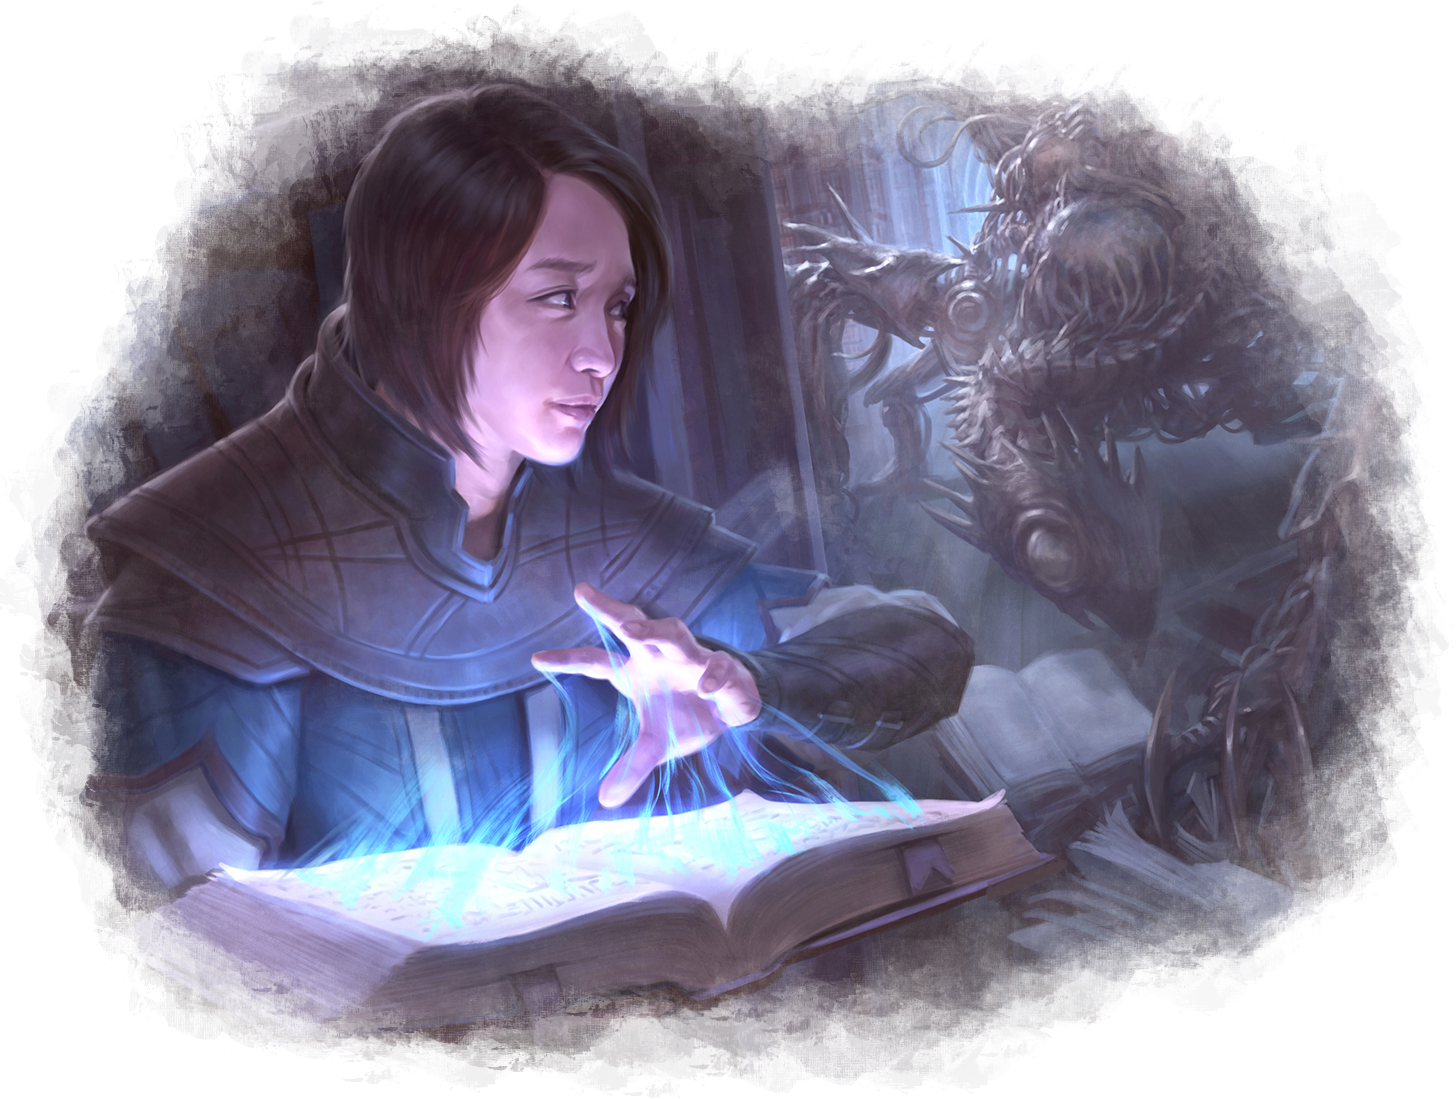
\includegraphics[width=0.525\paperwidth, keepaspectratio]{images/Advisor(4).png}};
		\addImageDBEntry{Page 5}{Art}{https://www.artofmtg.com/art/combat-research/}{Combat Research MtG Art from Dominaria United}{Justine Cruz}
	\end{tikzpicture}
	\vfill\eject
	
	\subparagraph*{Spells Known of 1st-Level and Higher}
	When you reach 3rd level, you learn three 1st-level wizard spells of your choice, two of which you must choose from the divination and enchantment spells on the wizard spell list.
	
	The Spells Known column of the Arcanology Spellcasting table shows when you learn more wizard spells of 1st level or higher. Each of these spells must be a divination and enchantment spell of your choice, and must be of a level for which you have spell slots. For instance, when you reach 7th level in this class, you can learn one new spell of 1st or 2nd level.
	
	The spells you learn at 8th, 14th, and 20th level can come from any school of magic.
	
	Whenever you gain a level in this class, you can replace one of the wizard spells you know with another spell of your choice from the wizard spell list. The new spell must be of a level for which you have spell slots, and it must be a divination and enchantment spell, unless you’re replacing the spell you gained at 3rd, 8th, 14th, or 20th level from any school of magic.
	
	\subparagraph*{Spellcasting Ability}
	Intelligence is your spellcasting ability for your wizard spells, since your magic comes from the same places as your knowledge of the world. You use your Intelligence whenever a spell refers to your spellcasting ability. In addition, you use your Intelligence modifier when setting the saving throw DC for a wizard spell you cast and when making an attack roll with one.
	
	\begin{center}
		\textbf{Spell Save DC} = 8 + your Proficiency Bonus + \\your Intelligence Modifier
	\end{center}
	\begin{center}
		\textbf{Spell Attack Modifier} = your Proficiency Bonus + \\your Intelligence Modifier
	\end{center}
	
	\begin{adjustwidth}{-1em}{-1.5em}\begin{ornamentedbox}
		\begin{DndTable}[width=\linewidth, header=The Arcanology Spellcasting\vspace*{-0.8\fontdimen6\font}]{YYYcccc}
			\textbf{Advisor Level}  &\textbf{Cantrips Known}	&\textbf{Spells Known}	&\makecell[c]{\\\\\textbf{1st}}	&\makecell[c]{\\\\\textbf{2nd}}	&\makecell[c]{\\\\\textbf{3rd}}	&\makecell[c]{\\\\\textbf{4th}}\\
			3rd		& 3	& 3		& 2		& --	& --	& --	\\
			4th		&3	&4		&3		&--	&--	&--	\\
			5th		&3	&4		&3		&--	&--	&--	\\
			6st		&3	&4		&3		&--	&--	&--	\\
			7nd		&3	&5		&4		&2	&--	&--	\\
			8rd		&3	&6		&4		&2	&--	&--	\\
			9th		&3	&6		&4		&2	&--	&--	\\
			10th	&4	&7		&4		&3	&--	&--	\\
			11th	&4	&8		&4		&3	&--	&--	\\
			12th	&4	&8		&4		&3	&--	&--	\\
			13th	&4	&9		&4		&3	&2	&--	\\
			14th	&4	&10		&4		&3	&2	&--	\\
			15th	&4	&10		&4		&3	&2	&--	\\
			16th	&4	&11		&4		&3	&3	&--	\\
			17th	&4	&11		&4		&3	&3	&--	\\
			18th	&4	&11		&4		&3	&3	&--	\\
			19th	&4	&12		&4		&3	&3	&1	\\
			20th	&4	&13		&4		&3	&3	&1	\\
		\end{DndTable}
		\begin{tikzpicture}[remember picture, overlay]
			\node[yshift=7.9cm, xshift=6.5cm, font=\bfseries\scriptsize] at (0,0) {\bfseries{- Spell Slots per Spell Level -}};
		\end{tikzpicture}
	\end{ornamentedbox}\end{adjustwidth}
	
	\subsubsection*{Word of Wizardry}
	\textnormal{\textit{3rd-Level Arcanology feature}}
	
	Your words carry immense weight, capable of unsettling even the most composed. You gain an additional application for your Word of Advice feature. You can now use your reaction whenever another creature that can hear you makes a d20 roll due to a spell you know.
	
	\subsubsection*{Convincing Words}
	\textnormal{\textit{6th-level Arcanology feature}}
	
	Your elegant words and enchanting gaze can magically enthrall another creature. When a creature that you can see within 30 feet of you fails a saving throw against your word of advice, it becomes charmed by you until the end of your next turn. The charmed creature’s speed drops to 0, and the creature is incapacitated and visibly dazed.
	
	On subsequent turns, you can spend an advice die and use your action to maintain this effect, extending its duration until the end of your next turn. However, the effect ends if you move more than 30 feet away from the creature, if the creature can neither see nor hear you, or if the creature takes damage.
	
	Once the effect ends, you can’t use this feature on that creature again until you finish a long rest.
	
	\subsubsection*{Malevolent Mockery}
	\textnormal{\textit{10th-level Arcanology feature}}
	
	When you cast vicious mockery, you can use your Word of Wizardry feature to grant the creature disadvantage on the save instead.
	
	In addition, you can spend 2 advice die to cast the spell as a reaction, given you haven't already used your action to cast the spell on your turn.
	
	\subsubsection*{Mastered Knowledge}
	\textnormal{\textit{14th-level Arcanology feature}}
	
	You gain proficiency with the Intelligence (Arcana) skill if you don’t already have it and gain advantage on any ability check that uses that proficiency.
	
	Additionally, when a creature within 30 feet of you succeeds on an Intelligence (Arcana) check, you regain 1 Advice Die.
	
	\subsubsection*{Tandem Targets}
	\textnormal{\textit{18th-level Arcanology feature}}
	
	Whenever a creature, including you, casts a spell targeting you, you can spend advice die, equal to the level of the spell being cast - if it is a cantrip, you still have to expend one die - to affect another creature with the spell. The caster must be able to hear you and the other creature must be within 30 feet and be able to see and hear you.
	\eject
	
	\subsection*{Archeology}
	By studying the remnants of historical civilizations and cultures Archaeologists uncover the past, forming a connection to the lives of those that came before, and unlocking within themselves a connection to history.
	
	\subsubsection*{Knowledge of Old}
	\textnormal{\textit{3rd-level Archeology feature}}
	
	You gain proficiency with a martial weapon and learn one language of your choice.
	
	\subsubsection*{Word of Authenticity}
	\textnormal{\textit{3rd-level Archeology feature}}
	
	Phrases of old can often bring back normalcy. You gain an additional application for your Word of Advice feature. Whenever a creature, other than you, rolls a d20 with advantage or disadvantage you can use your reaction to use your Word of Advice.
	
	\subsubsection*{Trap Sense}
	\textnormal{\textit{6th-level Archeology feature}}
	
	Dangerous secrets are only so for the unprepared, you're invaluable in such situations. As a bonus action on your turn you can sense the presence of any trap, within 30 feet. A trap, includes anything that would inflict a sudden or unexpected effect you consider harmful or undesirable, which was specifically intended as such by its creator. Thus, you would sense an area affected by the alarm spell, a glyph of warding, or a mechanical pit trap, but not natural instability or compromised infrastructure. You don't learn the location of each trap, but you do learn the general nature of the danger posed by a trap you sense.
	
	\subsubsection*{Exploring Eye}
	\textnormal{\textit{10th-level Archeology feature}}
	
	When you use the Search action and successfully find an obscured creature or object you become aware of the target's location while being within 60 feet of it. It does not gain any benefits of being hidden or invisible to you.
	
	\subsubsection*{Mastered Knowledge}
	\textnormal{\textit{14th-level Archeology feature}}
	
	You gain proficiency with the Intelligence (History) skill if you don’t already have it and gain advantage on any ability check that uses that proficiency.
	
	Additionally, when a creature within 30 feet of you succeeds on an Intelligence (History) check, you regain 1 Advice Die.
	
	\subsubsection*{Historian's Fallacy}
	\textnormal{\textit{18th-level Archeology feature}}
	
	There is much to be learned outside of the outdated scrolls and tomes. Whenever you use your Common Knowledge feature, you may choose an additional proficiency of any kind from a friendly creature, to grant to yourself and your companions.
	
	For example, if a creature has proficiency with martial weapons, you may grant yourself and up to 3 friendly creatures proficiency with martial weapons.
	
	\subsection*{Criminology}
	In the domain of Criminology, practitioners delve into the intricate study of criminal behavior and the resultant actions we know as crimes. These experts are masters of cunning and conniving, fearlessly taking on challenges of any scale and pursuing prizes of every magnitude. With an astute understanding of the criminal mind, they unravel mysteries and navigate the intricate web of deceit.
	
	\subsubsection*{Bonus Proficiencies}
	\textnormal{\textit{3rd-level Criminology feature}}
	
	You gain proficiency with thieves’ tools and learn the thieves’ cant language.
	
	\subsubsection*{Phony Pharynx}
	\textnormal{\textit{3rd-level Criminology feature}}
	
	You can unerringly mimic the speech patterns and voice of a creature that you hear speak for at least 1 minute, enabling you to pass yourself off as the creature or a native speaker of a particular land, provided that you know the language.
	
	\subsubsection*{Word of Privacy}
	\textnormal{\textit{3rd-level Criminology feature}}
	
	Advice given through secrets or shadow. You gain an additional application for your Word of Advice feature. Whenever another creature rolls a d20 while you are in dim-light or darkness, you can use your reaction to use the Word of Advice.
	
	\begin{tikzpicture}[remember picture, overlay]
		\node[opacity=1,inner sep=0pt, anchor=south west, yshift=-1.5cm, xshift=0cm] at (current page.south west){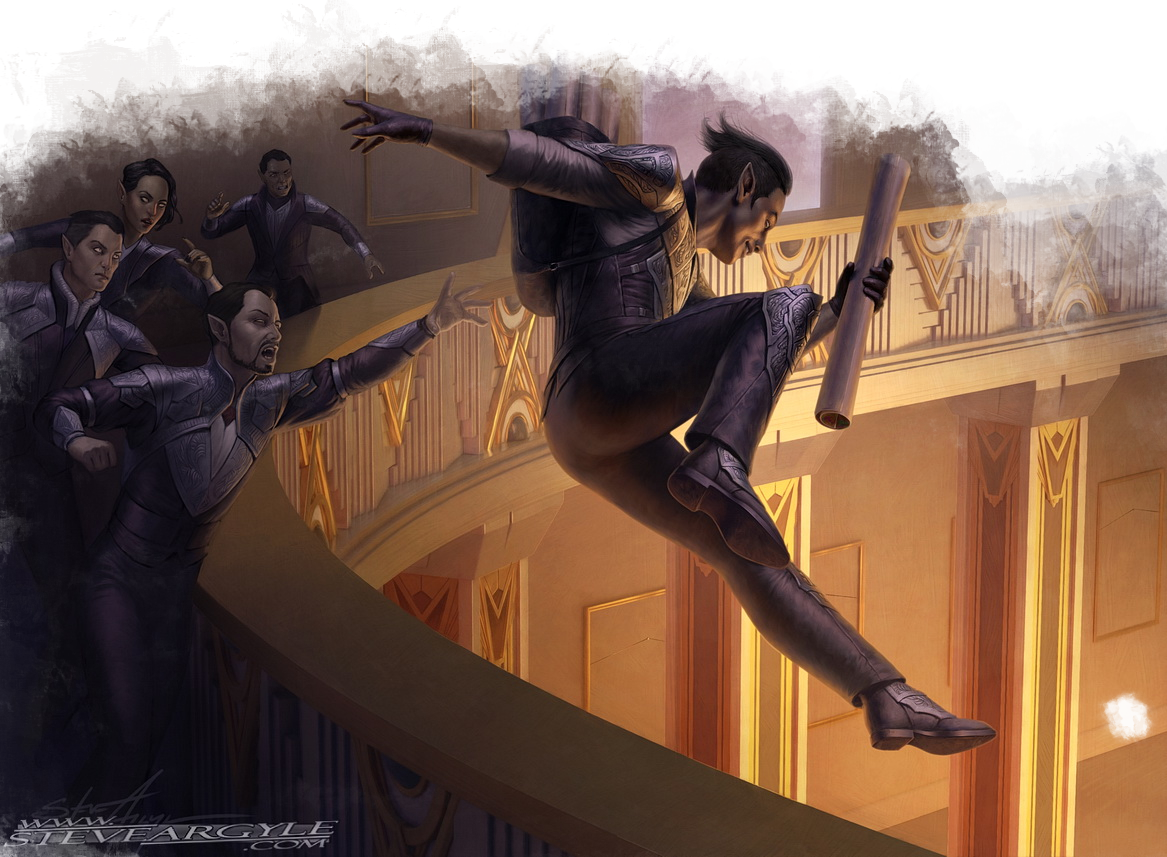
\includegraphics[width=\paperwidth, keepaspectratio]{images/Advisor(5).png}};
		\addImageDBEntry{Page 7}{Art}{https://www.artofmtg.com/art/rob-the-archives/}{Rob the Archives MtG Art from Streets of New Capenna}{Steve Argyle}
	\end{tikzpicture}
	
	\vfill\eject
	
	\subsubsection*{Uncanny Dodge}
	\textnormal{\textit{6th-level Criminology feature}}
	
	When an attacker that you can see hits you with an attack, you can use your reaction to halve the attack’s damage against you.
	
	\subsubsection*{Muscle Memory}
	\textnormal{\textit{10th-level Criminology feature}}
	
	Your study or practice of sleuth has come in handy. As a result, whenever you make a Dexterity check, you can treat a d20 roll equal to or lower than your Intelligence modifier to be equal to your modifier plus 1.
	
	\subsubsection*{Mastered Knowledge}
	\textnormal{\textit{14th-level Criminology feature}}
	
	You gain proficiency with the Intelligence (Investigation) skill if you don't already have it and gain advantage on any ability check you make that uses that proficiency.
	
	Additionally, when a creature within 30 feet of you succeeds on a Intelligence (Investigation) check, you regain 1 Advice Die.
	
	\subsubsection*{Auditory Secrecy}
	\textnormal{\textit{18th-level Criminology feature}}
	
	When an enemy that can hear but not see you, fails a d20 roll, you regain 1 advice die.
	
	Additionally, when you use the Help action to aid an ally in attacking a creature, the target of that attack can be within 60 feet of you, rather than within 30 feet of you, if you are heavily obscured.
	\vfill\newpage
	\vspace*{-2.4\fontdimen6\font}
	\subsection*{Polemology}
	Polemology, is the multi-disciplinary study of war. Advisors who specialize in such an area have molded themselves into unrivaled tacticians and strategists. While not on the front lines, they are highly trained and skilled warriors in their own right.
	
	\subsubsection*{Bonus Proficiencies}
	\textnormal{\textit{3rd-level Polemology feature}}
	
	You gain proficiency with martial weapons and heavy armor.
	
	\subsubsection*{Utilitarian Toughness}
	\textnormal{\textit{3rd-level Polemology feature}}
	
	Your hit point maximum increases by 3, and it increases by 1 every time you gain an advisor level.
	
	\subsubsection*{Word of Authority}
	\textnormal{\textit{3rd-level Polemology feature}}
	
	Whether orders or commands, a good shout can make an impact. You gain an additional application for your Word of Advice feature. Whenever another creatures makes a weapon attack or damage roll you can use your reaction to use your Word of Advice.
	
	\subsubsection*{Extra Attack}
	\textnormal{\textit{6th-level Polemology feature}}
	
	You can attack twice, instead of once, whenever you take the Attack action on your turn.
	
	\subsubsection*{Tactical Retreat}
	\textnormal{\textit{10th-level Polemology feature}}
	
	Whenever you take the Disengage action on your turn, your walking speed increases by 10 feet until the end of your next turn. Additionally, the walking speed of any ally who starts their turn within 5 feet of you increases by 10 feet until the end of that turn.
	
	\subsubsection*{Mastered Knowledge}
	\textnormal{\textit{14th-level Polemology feature}}
	
	You gain proficiency with the Strength (Athletics) skill if you don’t already have it and gain advantage on any ability check that uses that proficiency.
	
	Additionally, when a creature within 30 feet of you succeeds on a Strength (Athletics) check, you regain 1 Advice Die.
	
	\subsubsection*{Actions Speak}
	\textnormal{\textit{18th-level Polemology feature}}
	
	On occasion an example is best set by oneself. As a bonus action on your turn, you can spend advice die to gain the following benefits, for 1 round per die spent:
	
	\begin{itemize}
		\item You gain a bonus to your AC equal to your Intelligence modifier (minimum of +1).
		\item You gain temporary hit points equal to the roll(s).
		\item You can use Intelligence instead of Strength or Dexterity for the attack and damage rolls.
		\item Whenever you score a critical hit with a weapon attack, you regain 1 advice die.	
	\end{itemize}
	
	\vfill\eject
	
	\begin{tikzpicture}[remember picture, overlay]
		\node[opacity=1,inner sep=0pt, anchor=south east, yshift=0cm, xshift=15cm] at (current page.south east){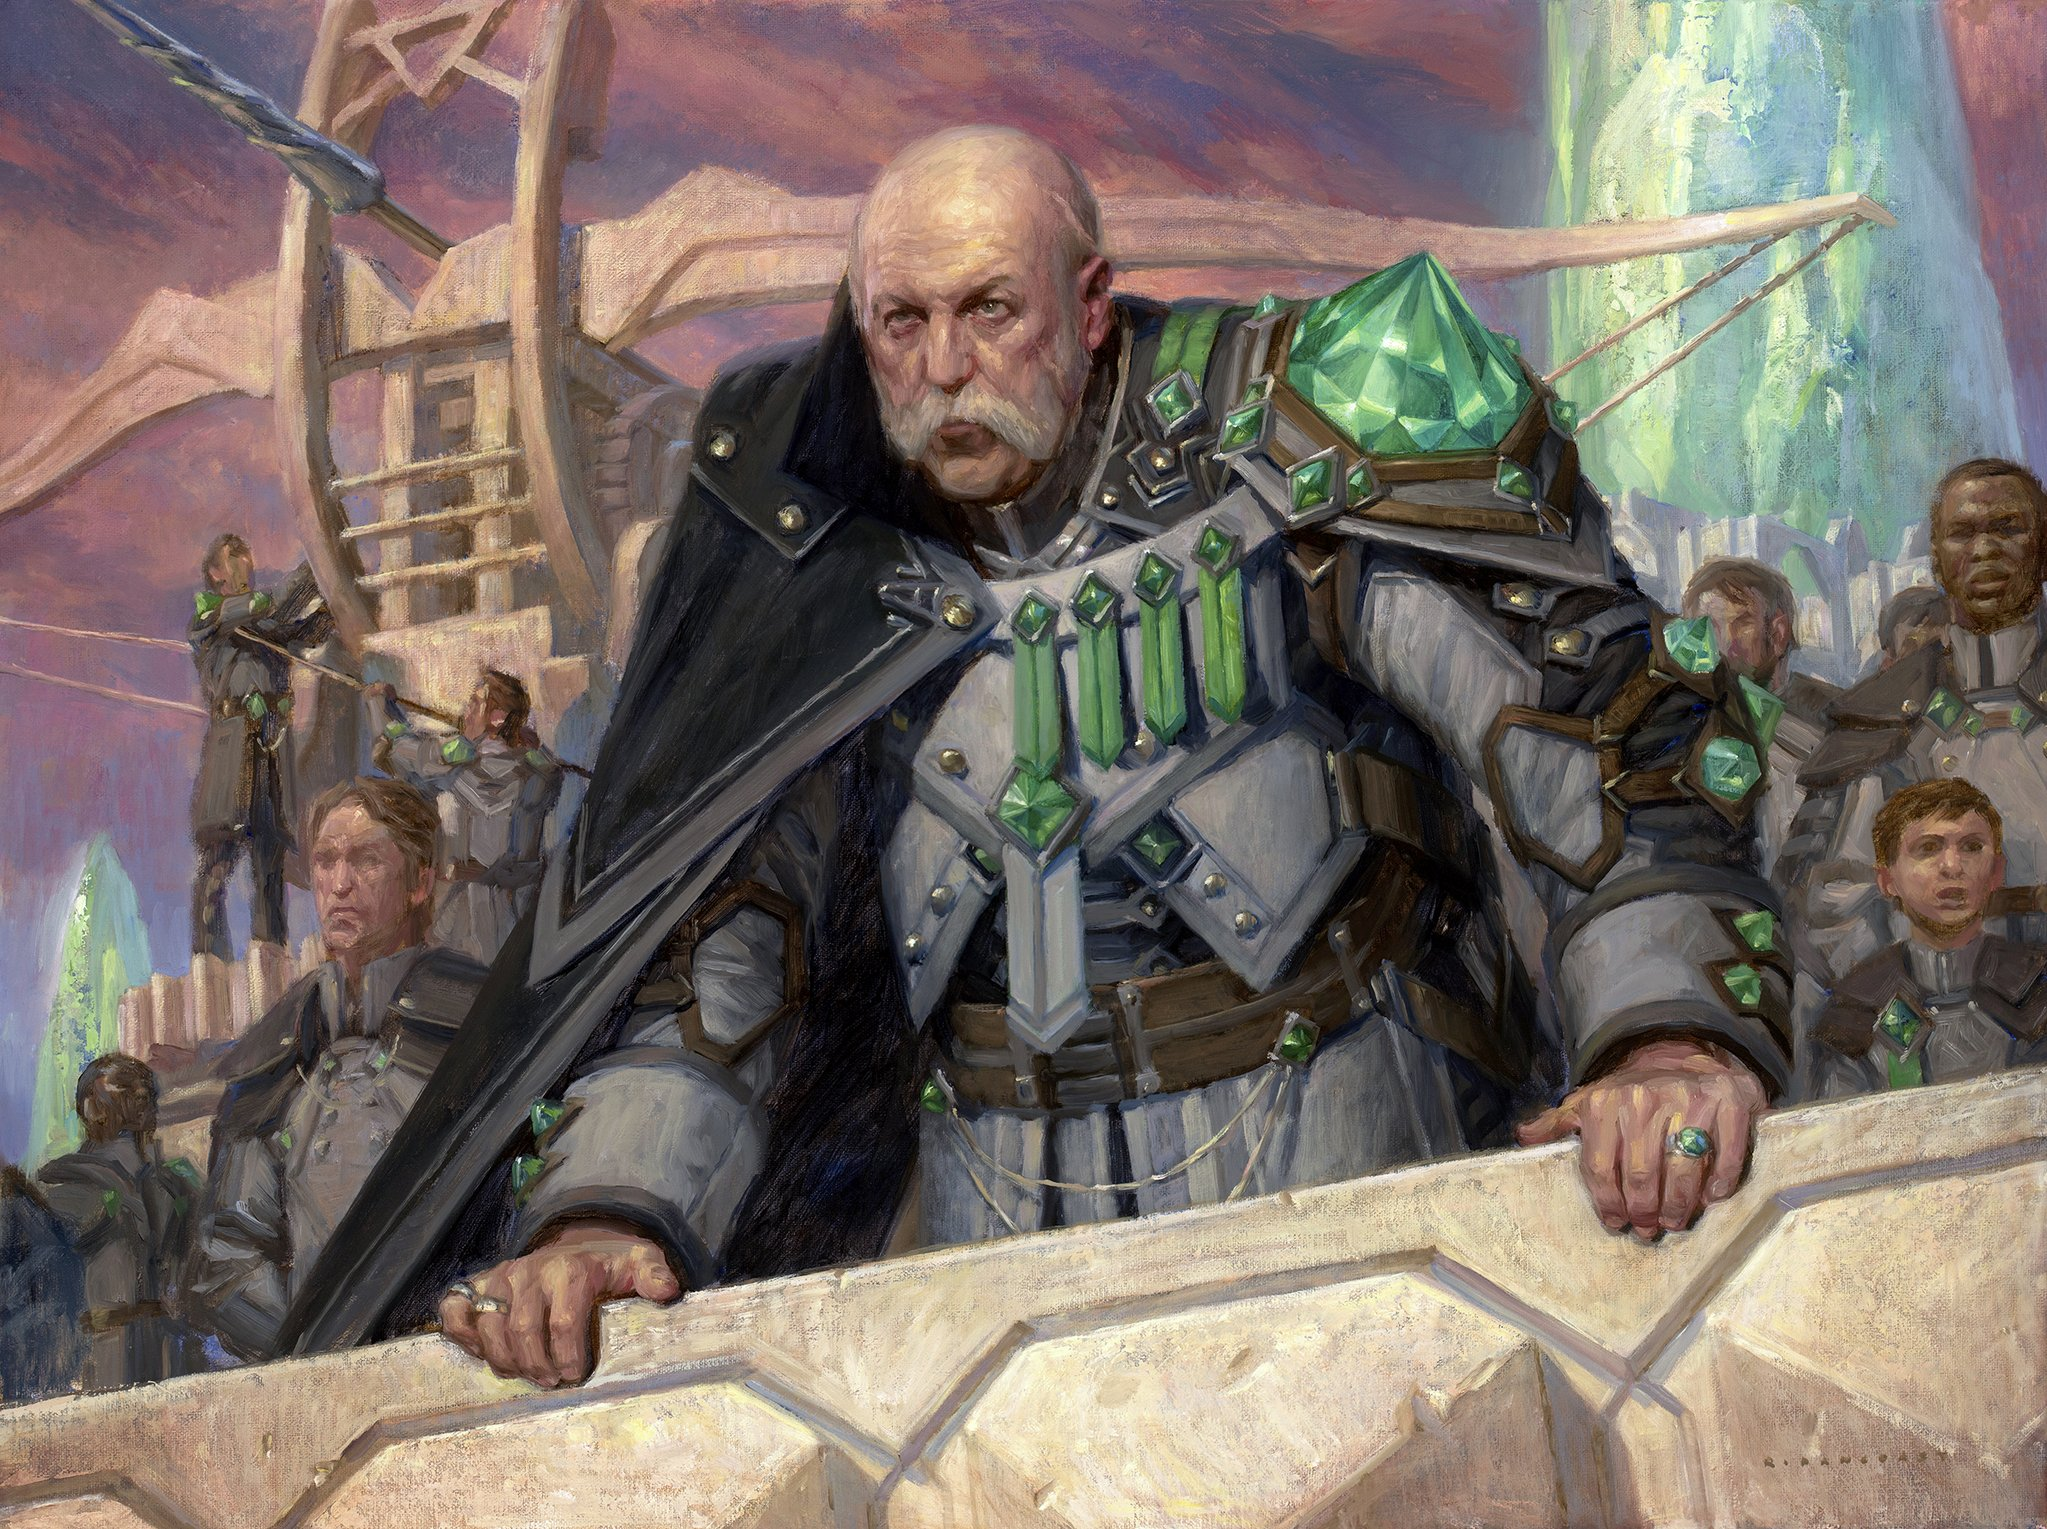
\includegraphics[height=\paperheight, keepaspectratio]{images/Advisor(6).png}};
		\addImageDBEntry{Page 8}{Art}{https://www.artofmtg.com/art/general-kudro-of-drannith/}{General Kudro of Drannith MtG Art from Ikoria}{Ryan Pancoast}
	\end{tikzpicture}
	
	\vfill\newpage
	
	\subsection*{Theology}
	The gods of the multiverse are truly a spectacle to behold. Many worship and pray to them in hopes for the gift of magic, but as only a true expert knows; there is more than magic can be studied.
	
	\subsubsection*{Researched Rituals}
	\textnormal{\textit{3rd-level Theology feature}}
	
	A gods magic isn't limited to only its clerics. You gain the ability to cast the augury and detect magic spells, but only as rituals, as described in the Spellcasting section.
	
	\subsubsection*{Word of Protection}
	\textnormal{\textit{3rd-level Theology feature}}
	
	The protection of their worshippers is incredibly important to the gods. You gain an additional application for your Word of Advice. Whenever another friendly creature within 30 feet of you is about to take damage, you can use your reaction to reduce the damage by the number rolled. All the other rules for Word of Advice still apply to you.
	
	\subsubsection*{Adroit of Old}
	\textnormal{\textit{6th-level Theology feature}}
	
	Gods often hold the key to the knowledge of old. When you use your Common Knowledge ability, you can choose one additional skill or tool proficiency that you have to grant onto other friendly creatures.
	
	\subsubsection*{Divine Dial}
	\textnormal{\textit{10th-level Theology feature}}
	
	A god's domain delineates their availability. You can cast the commune spell, but only as a ritual. When you do so, roll on the Divine Dial Table to determine which domain of deities you contact.
	
	\begin{tikzpicture}[remember picture, overlay]
		\node[opacity=1,inner sep=0pt, anchor=south west, yshift=-0.35cm, xshift=-0.15cm] at (current page.south west){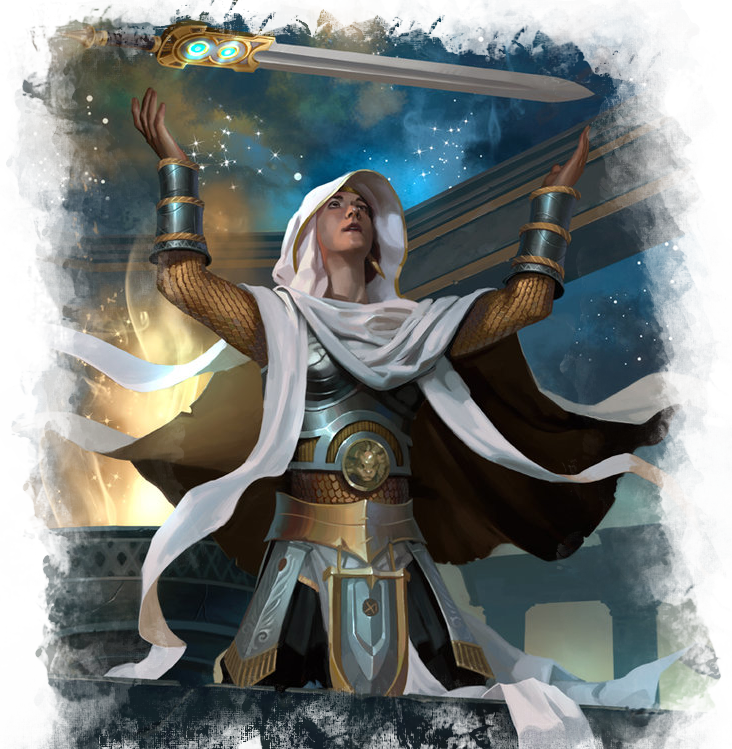
\includegraphics[width=0.55\paperwidth, keepaspectratio]{images/Advisor(7).png}};
		\addImageDBEntry{Page 9}{Art}{https://www.artofmtg.com/art/gods-willing/}{Gods Willing MtG Art from Theros}{Mark Winters}
	\end{tikzpicture}
	\vfill\eject
	
	\begin{ornamentedbox}
		\begin{DndTable}[width=\linewidth, header=Divine Dial Table]{lX}
			\textbf{d20}  &\textbf{Divine Domain}\\
			1		&Arcana Domain		\\
			2		&City Domain		\\
			3		&Death Domain		\\
			4		&Fate Domain		\\
			5		&Forge Domain		\\
			6		&Grave Domain		\\
			7		&Knowledge Domain	\\
			8-10	&Life Domain		\\
			11		&Light Domain		\\
			12		&Nature Domain		\\
			13		&Order Domain		\\
			14		&Peace Domain		\\
			15		&Protection Domain	\\
			16		&Tempest Domain		\\
			17		&Trickery Domain	\\
			18		&Twilight Domain	\\
			19		&War Domain			\\
			20		&Your Choice		\\
		\end{DndTable}
	\end{ornamentedbox}
	
	\subsubsection*{Mastered Knowledge}
	\textnormal{\textit{14th-level Theology feature}}
	
	You gain proficiency with the Intelligence (Religion) skill if you don’t already have it and gain advantage on any ability check that uses that proficiency.
	
	Additionally, when a creature within 30 feet of you succeeds on an Intelligence (Religion) check, you regain 1 Advice Die.
	
	\subsubsection*{Conduit of Divinity}
	\textnormal{\textit{18th-level Theology feature}}
	
	In an agreement with the gods, you have taken on some of their properties. You gain the following properties:
	
	\begin{itemize}
		\item You learn two Channel Divinities of your choice from those available to the cleric class. If a channel divinity requires your target to make a saving throw to resist its effects, the saving throw DC equals 8 + your proficiency bonus + your Intelligence modifier.
		\item You gain one use of Channel Divinity, and you regain it whenever you finish a short or long rest.
	\end{itemize}
	
	\subsection*{Zoology}
	Animals of all kinds are important to the world. Beasts, monstrosities and the like are deeply valued to an expert of Zoology. Often trusting in a pet of their own, these advisors utilize their knowledge of nature to assist.
	
	\subsubsection*{Animal Apprentice}
	\textnormal{\textit{3rd-level Zoology feature}}
	
	A well trusted assistant is common to find alongside a zoology expert. The animal apprentice is friendly to you and your companions, and it obeys your commands. See this creature’s game statistics in the Animal Apprentice stat block, which uses your proficiency bonus (PB) in several places.
	
	In combat, the apprentice shares your initiative count, but it takes its turn immediately after yours. It can move and use its reaction on its own, but the only action it takes on its turn is the Dodge action, unless you take a bonus action on your turn to command it to take another action. That action can be one in its stat block or some other action. If you are incapacitated, the apprentice can take any action of its choice, not just Dodge.
	
	If the apprentice dies, you can obtain a new apprentice by spending 8 hours bonding with a small or smaller beast that isn’t hostile to you.
	
	\subsubsection*{Word of the Wild}
	\textnormal{\textit{3rd-level Zoology feature}}
	
	The ebb and flow of nature is malleable to you. You gain an additional application for your Word of Advice. Whenever a beast, monstrosity, or plant makes a d20 roll you can use your reaction to use your Word of Advice.
	
	\subsubsection*{Above and Beyond}
	\textnormal{\textit{6th-level Zoology feature}}
	
	Sometimes the beast knows best. When your apprentice takes the Help action, you can expend an Advice Die for the apprentice to make an attack as a bonus action, using the number rolled in place of the normal damage of its strike.
	
	In addition, the apprentice's attacks now count as magical for the purpose of overcoming resistance and immunity to nonmagical attacks and damage.
	
	\subsubsection*{Increase Qualifications}
	\textnormal{\textit{10th-level Zoology feature}}
	
	A quality peer can come in all shapes and sizes. As an action on your turn, you and your animal apprentice both gain the following benefits for 1 minute:
	
	\begin{itemize}
		\item Your walking speeds increase by 10 feet.
		\item You can use the dash action as a bonus action.
		\item You gain an amount of temporary hit points equal to your advisor level, divided amongst both creatures.
		\item Once you use this feature, you must finish a short or long rest before you can use it again.
	\end{itemize}
	
	\subsubsection*{Mastered Knowledge}
	\textnormal{\textit{14th-level Archeology feature}}
	
	You gain proficiency with the Wisdom (Animal Handling) skill if you don’t already have it and gain advantage on any ability check that uses that proficiency.
	
	Additionally, when a creature within 30 feet of you succeeds on a Wisdom (Animal Handling) check, you regain 1 Advice Die.
	
	\subsubsection*{Unrivaled Assistance}
	\textnormal{\textit{18th-level Zoology feature}}
	
	Your apprentice was taught well so it became a master. When you or your apprentice take the Help action on your turn, the other creature can treat a d20 roll of 9 or lower as a 10.
	
	\eject
	
	\hfill\\\\
	\begin{DndMonster}[width=0.5\textwidth]{Animal Apprentice}
	    \DndMonsterType{Small Beast, neutral}
	
	    % If you want to use commas in the key values, enclose the values in braces.
	    \DndMonsterBasics[
	        armor-class = {13 + PB},
	        hit-points  = {5 + five times your advisor level (the companion has a number of Hit Dice [d8s] equal to your advisor level)},
	        speed       = {30 ft.},
	    ]
	    
		\renewcommand{\AbilityScoreSpacer}{~}
	    \DndMonsterAbilityScores[
	        str = 17,
	        dex = 17,
	        con = 15,
	        int = 12,
	        wis = 6,
	        cha = 6,
	    ]
	
	    \DndMonsterDetails[
	        saving-throws = {Dex +3 + PB, Con +2 + PB +5},
	        %skills = {Perception +4, Stealth +7},
	        %damage-vulnerabilities = {cold},
	        %damage-resistances = {bludgeoning, piercing, and slashing from nonmagical attacks},
	        %damage-immunities = {cold},
	        senses = {darkvision 60ft., passive Perception 11},
	        %condition-immunities = {frightened, poisoned},
	        languages = {understands the languages you speak},
	        %challenge = 2,
	    ]
	    
	    \DndMonsterSection{Actions}	
		\DndMonsterAttack[
	      name=Strike,
	      distance=melee, % valid options are in the set {both,melee,ranged},
	      %type=weapon, %valid options are in the set {weapon,spell}
	      mod=+3 + PB,
	      reach=5,
	      %range=20/60,
	      targets=one target,
	      dmg={1d8 + PB},
	      dmg-type={bludgeoning, piercing, or slashing (your choice)},
	      %plus-dmg=,
	      %plus-dmg-type=,
	      %or-dmg=,
	      %or-dmg-when=,
	      %extra=,
	    ]
	    
	    \DndMonsterSection{Actions}
	    \DndMonsterAction{Intercept Attack}
	    When a creature the companion can see hits a target with an attack, and the target is within 5 feet of the companion, the target instead takes half the damage. The companion takes the remainder of the damage.
	\end{DndMonster}
	
	\begin{tikzpicture}[remember picture, overlay]
		\node[opacity=1,inner sep=0pt, anchor=south east, yshift=1cm, xshift=2cm] at (current page.south east){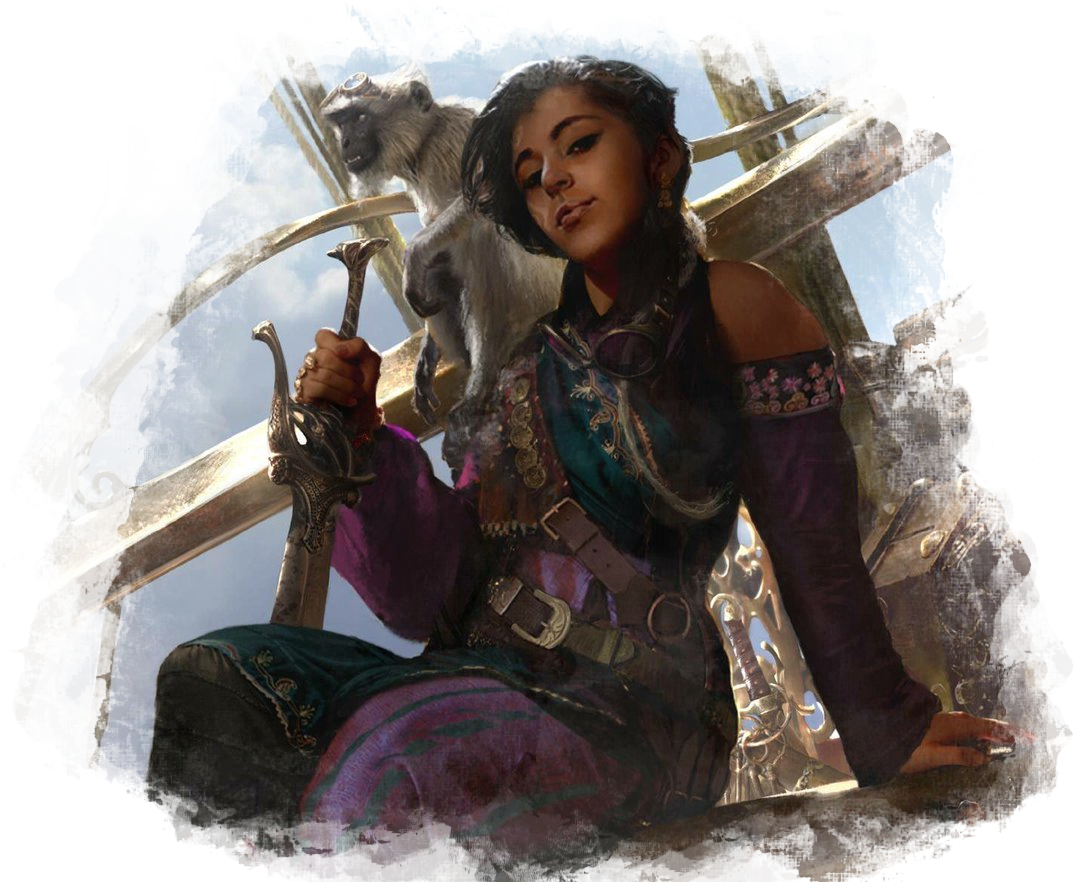
\includegraphics[width=0.65\paperwidth, keepaspectratio]{images/Advisor(8).png}};
		\addImageDBEntry{Page 10}{Art}{https://www.artofmtg.com/art/kari-zev-skyship-raider/}{Kari Zev, Skyship Raider MtG Art from Aether Revolt}{Brad Rigney}
	\end{tikzpicture}
	
	% Final Page
	\classesLastPage{images/backcover_Advisor.jpg}{0cm}{5cm}{height=\paperheight}{https://www.artstation.com/artwork/JvenZa}{The Enchanted Bibliotheca}{Nathanial Gibbs}{Created by Xcelar8 on GMBinder}
\end{document}